\section{Oferirea accesului unui utilizator}

\begin{figure}[H]
\begin{center}
  \subfloat[In cazul in care aplicatia este pornita, utilizatorul este redirectat in IncomingActivity]{\label{fig:useraddga}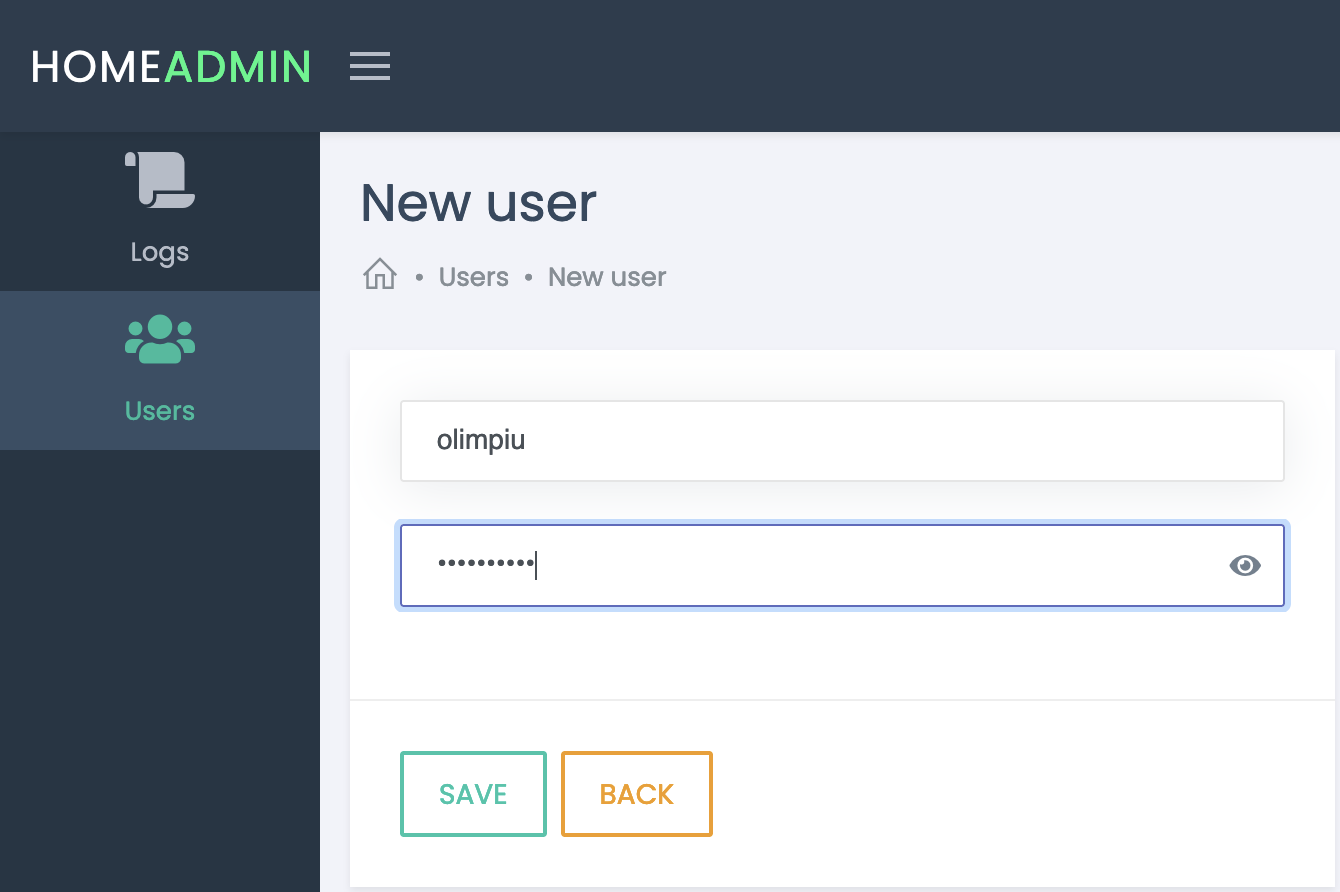
\includegraphics[width=\doublefigure]{05/06_admin_add_user.png}}
  \hfil
  \subfloat[In cazul in care aplicatia nu este in foreground, se trimite o notificare de sistem cu doua actiuni]{\label{fig:useraddgb}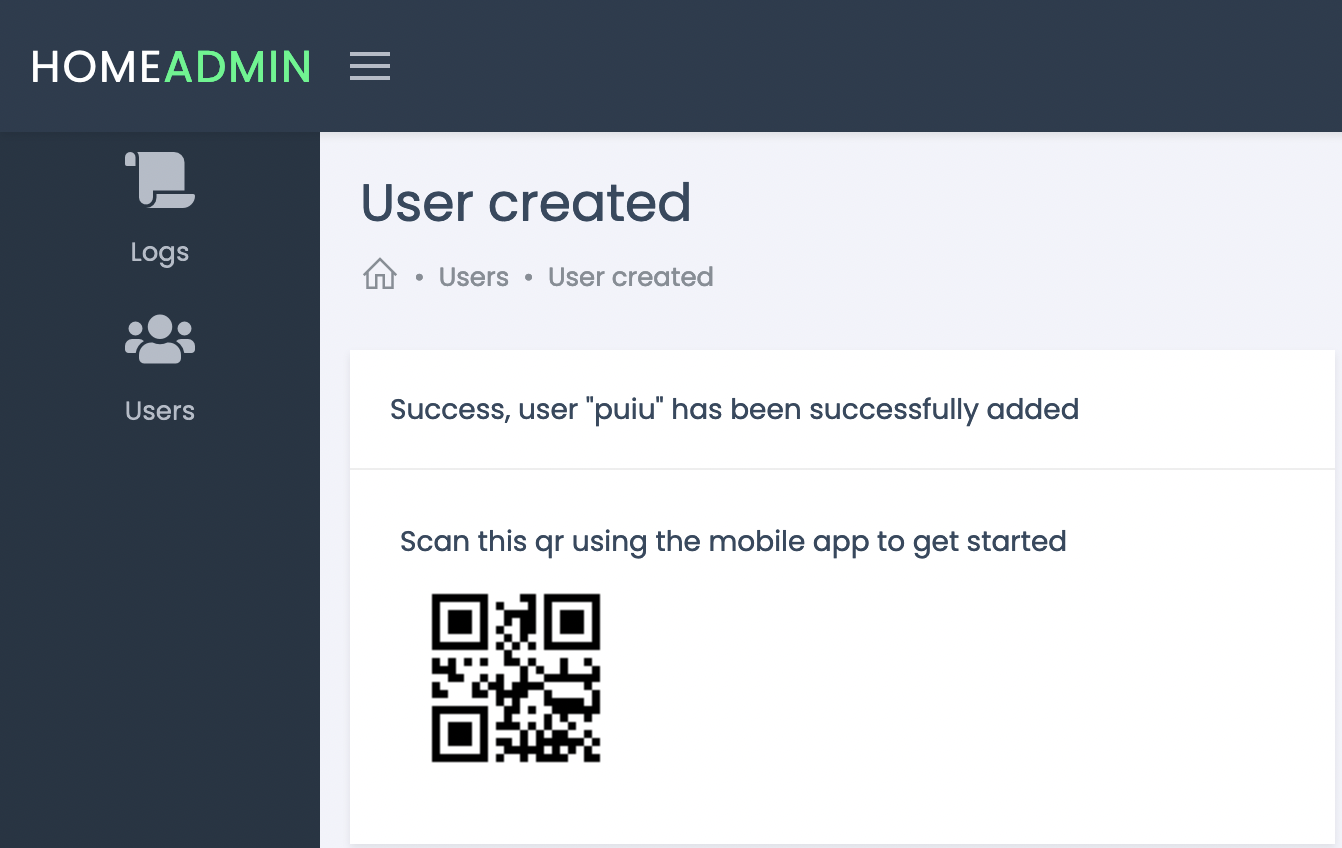
\includegraphics[width=\doublefigure]{05/07_admin_add_user_success.png}}
  \caption{Ecran apel}
  \label{fig:useraddg}
\end{center}
\end{figure}


\section{Raspuns automat}

Mi-am comandat pizza si ajunge in timp ce folosesc pistolul de lipit. Prin urmare voi programa interfonul sa raspunda si sa deschida automat usa la urmatorul apel.

\begin{figure}[H]
\begin{center}
  \subfloat[Apasarea butonului albastru auto-answer va arata meniul pentru configurarea functionalitatii]{\label{fig:autoanswera}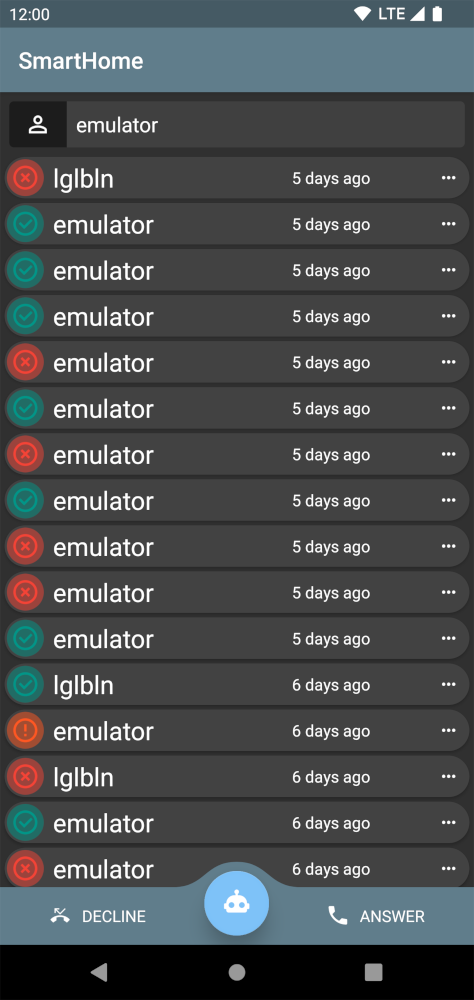
\includegraphics[width=\doublefigure]{05/01_android_autoanswer.png}}
  \hfil
  \subfloat[Alegerea unui interval pentru care functia va fi activa]{\label{fig:autoanswerb}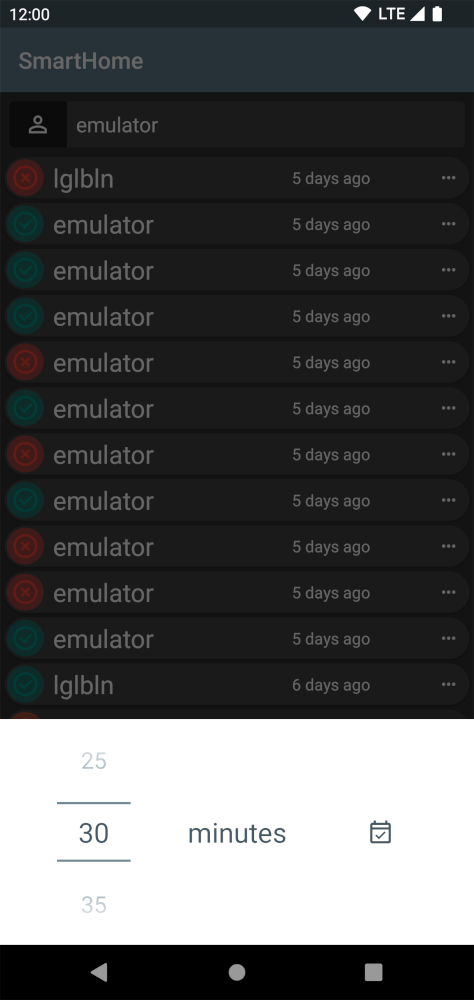
\includegraphics[width=\doublefigure]{05/02_android_auto_set.png}}
  \caption{Pasi pentru setare functie auto-answer}
  \label{fig:autoanswer}
\end{center}
\end{figure}

Se confirma ca functia este activata prin colorarea butonului auto-answer in portocaliu. Intr-o maniera similiara, daca se doreste oprirea inainte de termen, se poate face acest lucru din meniul anterior.

\section{Raspuns de la distanta}

Mi-am pierdut cartela standard \acrfull{rfid} pentru a intra in bloc. Asadar, voi suna la numerul apartamentului meu si voi folosi aplicatia mobila pentru a raspunde la propriul apel.

\begin{figure}[H]
\begin{center}
  \subfloat[In cazul in care aplicatia este pornita, utilizatorul este redirectat in IncomingActivity]{\label{fig:ringinga}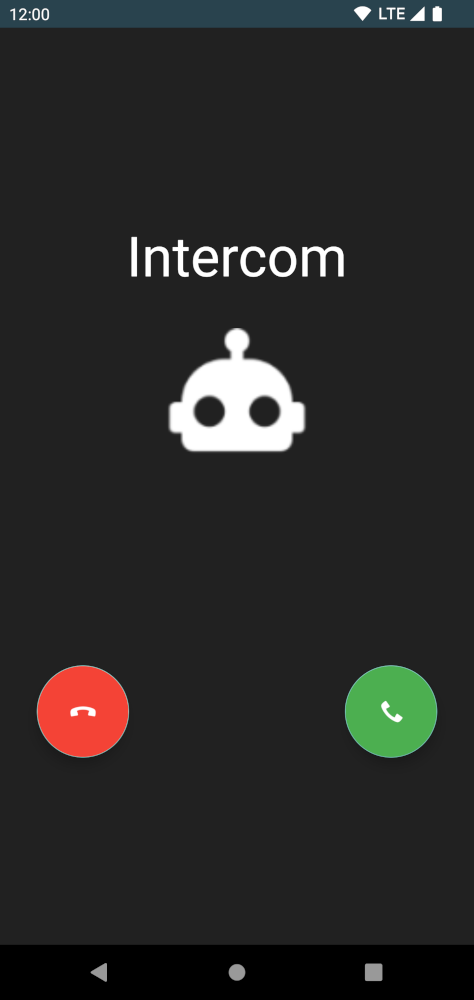
\includegraphics[width=\doublefigure]{05/04_android_app_ringing.png}}
  \hfil
  \subfloat[In cazul in care aplicatia nu este in foreground, se trimite o notificare de sistem cu doua actiuni]{\label{fig:ringingb}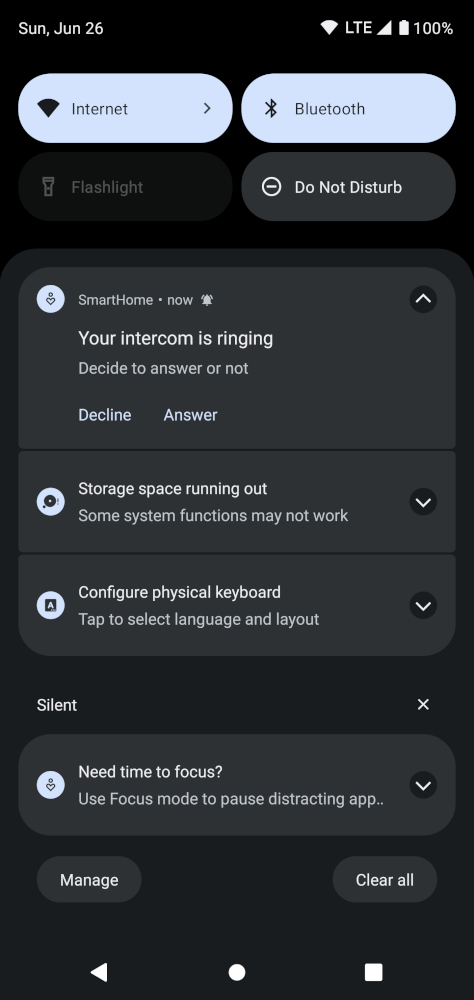
\includegraphics[width=\doublefigure]{05/05_android_notification_ringing.png}}
  \caption{Ecran apel}
  \label{fig:ringing}
\end{center}
\end{figure}

O alta varianta pentru mitigarea acestei probleme a fost folosirea unui tag \acrfull{nfc} care contine codat url-ul de acces impreuna cu un token care nu expira. Astfel prin scanarea lui cu un telefon ce dispune de anena \acrshort{nfc} se va realiza request-ul din browserul default al utilizatorului, rezultand in deschiderea interfonului.